
\section{Przygotowanie danych}

Obszerny zbiór danych jest kluczowym elementem systemów głębokiego uczenia,
ponieważ właśnie na podstawie danych model rozwiązuje problem.
Dane składają się z nagrań audio i odpowiadających im transcrypcji.
Brakuje ogólnodostępnych zbiorów danych, a w szczególności dotyczących języka polskiego.
Jednym z nielicznych ogólnodostępnych zbiorów danych jest zbiór \emph{Clarin-PL}\cite{pjatk_corpus}, który pochodzi
z ogólnoeuropejskiej inicjatywy \emph{Common Langugage Resources and Technology Infrasctructure (CLARIN)}.
Zbiór treninowy \emph{Clarin-PL} posiada 34 godziny oznaczonych nagrań.
Jest to niewielka ilść w porównaniu do ogólnodostępnych zbiorów języka anglielskiego.
Na podstawie innych źródeł m.in. zbiór \emph{Jurisdic}\cite{dataset_jurisdic} zebrano dodatkowo 364 godzin\ref{table:datasets}.

\begin{table}[h!]
\centering
 \begin{tabular}{l c c}
  \toprule
  Zbiór danych & Rozmiar (godz.) & Liczba próbek (tyś.) \\
  \midrule
  Clarin-PL & 34  & 41 \\
  Inne & 351 & 578 \\
  \bottomrule
 \end{tabular}
\caption{
Dostępne zbiory danych.
Liczba próbek po segmentacji.}
\label{table:datasets}
\end{table}

Zbiór danych zebrany z różnych źródeł jest silnie niejednorodny.
Liczba słów w nagraniach jest w przedziale od jednego do nawet kilkudziesięciu.
Na całym zbiorze dokonano segmentacji na pojedyncze wyrazy.
Następnie połączono wyrazy w próbki od 3 do 7 wyrazów włącznie.
Na rysunku \ref{fig:data_histograms} przedstawiono dystrybucję długości próbek w zbiorach,
które są zbliżone.
Rozkład 1- i 2-gramów liter w obu zbiorach jest podobny, co wskazuję na podobny rozkład
trudnych przykładów pod względem gramatycznym.
Długości próbek \emph{Clarin-PL} są nieznacznie dłuższe pod wzlędem zarazówno ilości wyrazów jak i długości nagrania.
Wszystkie nagrania jedo i dwu wyrazowe odrzucono, ze względu na szum w nich wsytępujący.
Dobranie danych silnie definiuje cały proces uczenia, jak również możliwości modelu.
Trenowanie arbitralnie długich próbek jest możliwe, ale wymaga większej uwagi podczas trenowania
i jest dodatkowym wyzwaniem.
W zbiorze treningowym znalazło się ponad 600 tyś. próbek \ref{table:datasets}.
Wszystkie próbki dźwiękowe posiadają pojedynczy kanał (mono) o częstotliwości próbkowania 16 kHz z głębią 16 bitów.

\begin{figure}
    \centering
    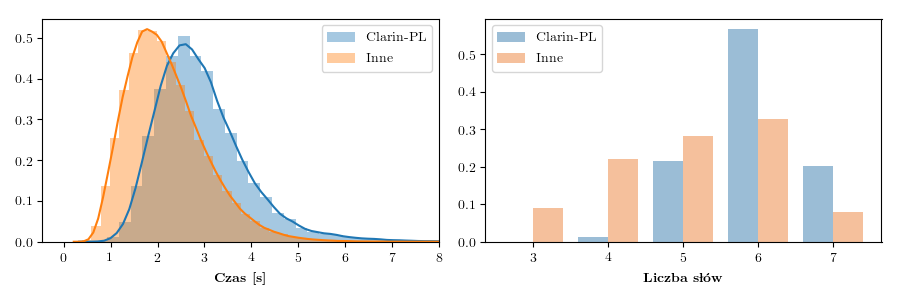
\includegraphics[width=12cm]{figures/data-histogram.png}
    \caption{Histogramy, po lewej długość próbek w sekundach i po prawej ilość wyrazów}
    \label{fig:data_histograms}
\end{figure}

Dane wejściowe do modelu to sygnał audio przedstawiono w posiaci \emph{Mel Frequency Cepstral Coefficients (MFCC)}.
Alternatywną reperzentacją jest obliczenie energii w poszczególnych pasmach spectogramu.
Dzięki MFCC spectogram jest skompresowany, co w konsekwencji powoduję zmniejszenie liczby parametrów modelu.
Użycie MFCC jest uzastadnione w zadaniu rozpoznawania mowy, w którym szczegółowa charaterystyka widma
nie jest ważna (w przeciwieństwie do speaker recognition).
W tabeli \ref{table:mfcc} przedstawiono wykorzystane parametry MFCC.
Szczególnie szerokość okienka i krok może zmieniać się w zależności od charakterystyki przetwarzanego języka,
w tym przypadku języka polskiego.

\begin{table}[h!]
\centering
 \begin{tabular}{c c c}
  \toprule
  Preemphasis & Winlen (ms) & Winstep (ms) & Winfunc & NFFT & Numfil & Numcep & Ceplifter\\
  \midrule
  0.95  &  32  &  20  & hamming & 512 & 26 & 26 & 22
  \bottomrule
 \end{tabular}
\caption{
Parametry wykorzystane do obliczania MFCC: współczynnik wzmocnienia, szerokość okienka, krok okienka,
funkacja okienkowa, szerokość transformaty, liczba filterbank energies, liczba MFC Coefficients, cepstral lifter (wzgmocnienie wyższych częstotliwości DCT).}
\label{table:mfcc}
\end{table}

Dane treningowe zostały znormalizowane tak, aby poziom całkowitej energi próbki pozostał niezmienny.
Z każdego MFC Coefficient usunięto globalną średnią całego zbioru treningowego tej cechy oraz podzielono poprzez
globalne odchylenie standardowe.
Podobny efekt można uzyskać wykorzystująć \emph{Batch Normalization} na danych wejściowych.
Wszystkie próbki zostały zapisane w pliku HDF5 tak, aby szybko były dostępne podczas optymalizacj.
Warto zobaczyć implementacje skryptów `features.py` oraz `features_norm.py`.
